\documentclass[a4paper,twoside]{article}
\usepackage[dvipsnames]{xcolor}
\usepackage{a4wide,graphicx,fancyhdr,amsmath,amssymb,csquotes,caption, subcaption, url,hyperref,booktabs,longtable,rotating,array,tikz,relsize,xspace,tabularx}
\usepackage[english]{babel}
\usepackage[backend=biber, maxbibnames=10]{biblatex}
\usepackage[colorinlistoftodos]{todonotes}
\usepackage{regexpatch}
\usepackage{tikzit}
\newcolumntype{R}[1]{>{\begin{turn}{90}\begin{minipage}{#1}\small}l%
	<{\end{minipage}\end{turn}}%
	}

\protected\def\omnet{OMNeT\nolinebreak[4]\hspace{-.05em}\raisebox{.4ex}{\relsize{-3}{\textbf{++}}}\xspace}

\makeatletter
\xpatchcmd{\@todo}{\setkeys{todonotes}{#1}}{\setkeys{todonotes}{inline,#1}}{}{}
\NewBibliographyString{artno}
\DefineBibliographyStrings{english}{artno = {Art\adddotspace No\adddot}}

\DeclareFieldFormat[article,periodical]{eid}{\bibstring{artno}\addabbrvspace #1}

\addbibresource{resources.bib}
%------------------------- Colour definitions --------------------------
\definecolor{lightblue}{HTML}{77AADD}
\definecolor{lightcyan}{HTML}{99DDFF}
\definecolor{mint}{HTML}{44BB99}
\definecolor{pear}{HTML}{BBCC33}
\definecolor{olive}{HTML}{AAAA00}
\definecolor{lightyellow}{HTML}{EEDD88}
\definecolor{orange}{HTML}{EE8866}
\definecolor{pink}{HTML}{FFAABB}
\definecolor{palegrey}{HTML}{DDDDDD}
%--------------------------------- Tikz ---------------------------------
\usetikzlibrary{positioning}
\usetikzlibrary{shapes.geometric}


\input{sample.tikzstyles}
%------------------------ Macros and Definitions ------------------------

\setlength\headheight{20pt}
\addtolength\topmargin{-10pt}
\addtolength\footskip{20pt}

\fancypagestyle{plain}{%
\fancyhf{}
\fancyhead[LO,RE]{\sffamily\bfseries\large }
\fancyhead[RO,LE]{\sffamily\bfseries\large 2IMC0 Preparation Graduation Project ES}
\fancyfoot[LO,RE]{\sffamily\bfseries\large department of mathematics and computer science}
\fancyfoot[RO,LE]{\sffamily\bfseries\thepage}
\renewcommand{\headrulewidth}{0pt}
\renewcommand{\footrulewidth}{0pt}
}

\pagestyle{fancy}
\fancyhf{}
\fancyhead[RO,LE]{\sffamily\bfseries\large }
\fancyhead[LO,RE]{\sffamily\bfseries\large 2IMC0 Preparation Graduation Project ES}
\fancyfoot[LO,RE]{\sffamily\bfseries\large department of mathematics and computer science}
\fancyfoot[RO,LE]{\sffamily\bfseries\thepage}
\renewcommand{\headrulewidth}{1pt}
\renewcommand{\footrulewidth}{0pt}

%--------------------------------- Text ----------------------------------

\begin{document}
	\pagenumbering{roman}
	\begin{titlepage}

\newcommand{\HRule}{\rule{\linewidth}{0.5mm}} % Defines a new command for the horizontal lines, change thickness here

\center % Center everything on the page
 
%----------------------------------------------------------------------------------------
%	HEADING SECTIONS
%----------------------------------------------------------------------------------------

\includegraphics[width=0.55\textwidth]{images/tuelogonew.png}\\[0.7cm]
\textsc{\LARGE Eindhoven University of Technology}\\[2.5cm] % Name of your university/college

%----------------------------------------------------------------------------------------
%	TITLE SECTION
%----------------------------------------------------------------------------------------

\HRule \\[0.4cm]
{ \huge \bfseries Preparation Graduation Project ES}\\[0.4cm] % Title of your document
2IMC05
\HRule \\[2cm]
 
%----------------------------------------------------------------------------------------
%	AUTHOR SECTION
%----------------------------------------------------------------------------------------

\begin{minipage}[t]{0.5\textwidth}
\begin{flushleft} \large
\emph{Author:}\\
Stephan P.O \textsc{Oostveen}\\
\end{flushleft}
\end{minipage}
~
\begin{minipage}[t]{0.39\textwidth}
\begin{flushright} \large
\emph{Graduation supervisor:} \\ 
Pieter J.L \textsc{Cuijpers}\\  % Supervisor's Name
\end{flushright}
\end{minipage}\\[4cm]

% If you don't want a supervisor, uncomment the two lines below and remove the section above
%\Large \emph{Author:}\\
%John \textsc{Smith}\\[3cm] % Your name

%----------------------------------------------------------------------------------------
%	DATE SECTION
%----------------------------------------------------------------------------------------
{\large \today}\\[3cm] % Date, change the \today to a set date if you want to be precise

%----------------------------------------------------------------------------------------

\vfill % Fill the rest of the page with whitespace

\end{titlepage}
	\tableofcontents
	\newpage
	\pagenumbering{arabic}
	\section{Introduction}
\label{sec:introduction}
Lightyear designs and develops solar electric vehicles (SEVs), these are highly efficient battery electric vehicles that can charge their batteries using an integrated solar panel. The following factors play a role in a vehicle's efficiency: Aerodynamic drag, friction losses from tires, cabin heating and cooling, drivetrain losses, static energy consumption. Lightyear seeks to design a vehicle that minimizes these losses as a reduction in energy consumption has a snowball effect on vehicle efficiency. For example, a lower aerodynamic drag enables the use of a smaller battery pack while maintaining the same range, reducing the vehicle weight, resulting in less friction losses from the tires etc. In the end yielding a very efficient vehicle that can charge at any time using the power of the sun. Lightyear is constantly searching for solutions which improve vehicle efficiency, one key aspect which can be optimized is the electrical/electronic architecture.

\subsection{Current and future automotive architectures}
\label{sec:automotive-arch}
Modern vehicles are mostly electrically/electronically controlled, ranging from basic functionality such as acceleration (throttle pedal) and lighting to more advanced features such as ride height control and Autonomous Emergency Braking System. The number of electrically/electronically controlled features has grown over time by adding several electronic control units (ECUs) per feature to an already existing decentralized control architecture. This means that multiple ECUs need to communicate in order to achieve a certain function. As a result modern vehicles can contain more than 100 ECUs~\cite{bandur2021making} and several communication networks. This has several drawbacks: increased communication load on the in-vehicle network(s), increased cost due to the large number of ECUs and large wiring harness, increased software complexity, more software variants, higher maintenance costs and reduced reliability~\cite{bandur2021making}. An example of such a decentralized architecture is shown in Figure~\ref{fig:functional-arch}, the blue rectangles represent ECUs, ECUs that are part of a single function or domain (body control, drivetrain etc) are connected to each other with an automotive network such as LIN or CAN. The functions or domains work together by means of a gateway (red rectangle) which bridges or translates messages to and from the different networks. Sometimes certain ECUs are also connected to more than one network for practical reasons such as the Steering column ECU in the example.

\begin{figure}[htb]
    \centering
    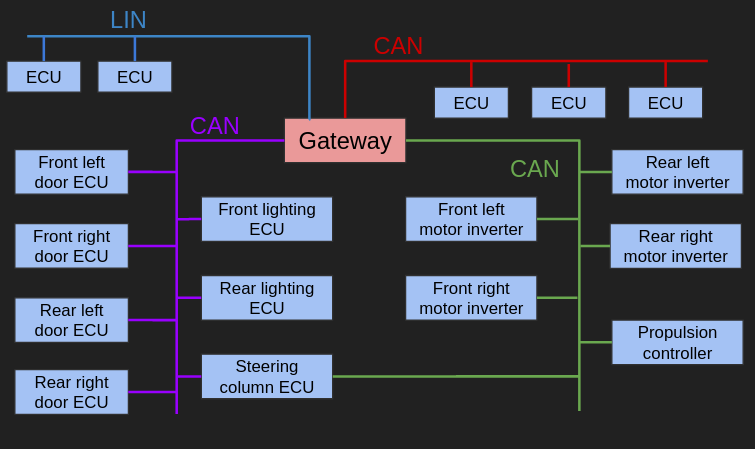
\includegraphics[width=\textwidth]{images/functional-arch.png}
    \caption{Example of an automotive decentralized control architecture}
    \label{fig:functional-arch}
\end{figure}

The automotive industry has recognized these issues and is moving towards a centralized control architecture with one large ECU per physical zone, called a zonal architecture~\cite{ashjaei2021time}. Instead of having many small ECUs performing only one part of a function there will be one central ECU responsible for all the control functions and a few large ECUs (zone ECUs) strategically placed in the car executing the commands of the central controller. To reduce complexity, weight and cost even more the zone ECUs are networked through a single high bandwidth, low latency network instead of the multiple low bandwidth networks running through a vehicle nowadays. The zone ECUs can act as a bridge for legacy networks used by legacy components in the physical neighbourhood. An example is depicted in Figure~\ref{fig:zonal-arch}.

In the zonal architecture the zone ECUs and central controller are connected through a high bandwidth low latency network, automotive Ethernet together with Time Sensitive Networking (TSN) have been chosen as the key networking technologies. The choice for automotive Ethernet is supported by the work of the Time Sensitive Networking (TSN) Task Group of the IEEE 802.1 Working Group, which allow real-time communication over IEEE 802.3 (Ethernet) networks~\cite{klaus2019zonal}. Other relevant factors are the high bandwidth capabilities relative to traditional networking technologies such as CAN and FlexRay, Internet Protocol (IP) based end to end communication support, automotive specific physical layer standards for various data rates and standardization by the IEEE~\cite{ashjaei2021time}.

Figure~\ref{fig:zonal-arch} represents the same vehicle as in Figure~\ref{fig:functional-arch} with a zonal architecture. The number of ECUs, including gateway, is reduced from 18 in the decentralized architecture to 11 in the zonal architecture. This reduction has been achieved by consolidating several ECUs into the zone ECUs, reducing mass. The number of networks has stayed the same, three CAN networks and one LIN network in the decentralized control architecture versus 3 CAN networks and one Ethernet network in the zonal architecture. But crucially the physical wiring loom has been simplified in the zonal architecture as there is only one network cable spanning the entire vehicle length. This simplification reduces weight, since there is only one cable going from the back to the front instead of two or more. Additionally, the shorter sub-wire harnesses can be manufactured automatically, reducing costs.

\begin{figure}[htb]
    \centering
    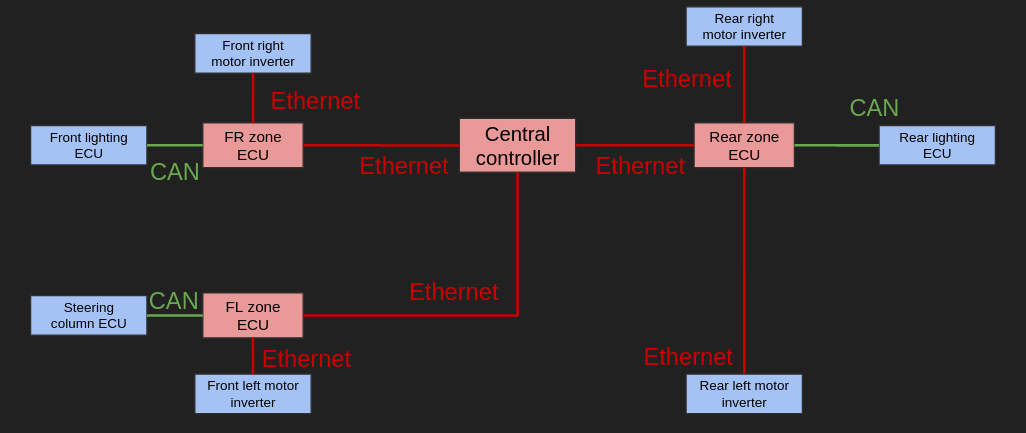
\includegraphics[width=\textwidth]{images/zone-arch.png}
    \caption{Example of an automotive zonal architecture}
    \label{fig:zonal-arch}
\end{figure}

\subsection{Real-time communication over Ethernet}
Some electrically/electronically features in a vehicle pose strict timing requirements on the architecture and implementation. For example the passenger safety system must always deploy the airbags within a specific time period after a crash. Deploying the airbags too quickly or too late can cause harm to the passengers. Systems with strict timing guarantees are called real-time systems and require the timing properties of the system to be bounded and analysable. If the implementation of such a feature requires several networked ECUs to work together the network and the ECUs should be real-time. Examples of automotive networks that support real-time communication are LIN, CAN and FlexRay. 

IEEE 802.3 Ethernet is not a real-time network, one of the original design philosophies is best-effort transmission of frames~\cite{metcalfe1976ethernet}. The idea being that it would be not economically viable to create a network that guarantees error-free message delivery. Putting the responsibility of dealing with the various possible errors, such as packet loss, duplication, large delays etc, on the communicating processes. This allows giving good average-case performance to a large group of users in an economically viable way, but sacrifices the real-time property. 

Originally Ethernet was designed as a bus network with CSMA/CD to allow multiple hosts to use a shared medium. CSMA/CD is also used as a Medium Access Control method in "modern" twisted-pair Ethernet networks where multiple nodes are in the same collision domain, for example when using half-duplex communication or when repeater hubs are used to interconnect Ethernet segments. CSMA/CD violates the real-time property because it uses a randomized exponential backoff algorithm when retransmission of frames is necessary due to simultaneous transmission by distinct nodes in the collision domain. This means that frames can be delayed a random amount of time. How often a message is delayed increases as the network load increases.

Full-duplex switched Ethernet no longer uses CSMA/CD, but the switches introduce a delay as well. IEEE 802.3 does not specify how a switch should operate, hence no guarantee can be made about the queuing and switching delay added to the transmission time by a switch. Lastly, it is reasonable to assume that queuing delays increase as the number of packets passing through a switch increases. Together this makes Ethernet unsuitable for use in a real-time system. 

Several higher level protocols have been proposed to make real-time communication on top of Ethernet possible e.g. EtherCAT, PROFINET, TTEthernet and Time Sensitive Networking. Some of these protocols require special network interface cards or switches to operate, or they are not directly interoperable with \textit{standard} Ethernet which complicates mixing the network with other devices such as a computer using the TCP/IP stack. 

\subsection{Time Sensitive Networking}
\label{sec:tsn}
As mentioned in Section~\ref{sec:automotive-arch}, Time Sensitive Networking (TSN) is a set of standards created by an IEEE Task Group according to their website their goal is "\textit{to provide deterministic connectivity through IEEE 802 networks, i.e., guaranteed packet transport with bounded latency, low packet delay variation and low packet loss}". TSN standards and amendments to standards can be grouped in four categories according to their design goal~\cite{ashjaei2021time}: Timing and synchronization, resource management, bounded low latency and high reliability.

\paragraph{Globally accurate time base}
TSN recognized that having an accurate common notion of time in a network simplifies the design and implementation of real-time systems. A globally accurate and synchronized time base is the central concept in the Time Triggered Architecture~\cite{kopetz2003time} from which TTEthernet was developed. The IEEE 802.1AS-2020 standard specifies an algorithm, called the Best Master Clock Algorithm (BMCA), for determining the time reference node (Grand Master) in the network. The generalized precision time protocol (gPTP) takes care of synchronizing the clocks of all nodes by supplying the Grand Master clock value. It also provides redundancy in the clock synchronization and Grand Master clock in case of node or link failure.

\paragraph{Network resource management} In cases where real-time network traffic has a dynamic nature e.g., an audio/video stream in a converged network which only occurs at specific times, TSN provides the Stream Reservation Protocol (SRP) through the IEEE 802.1Qat standard. SRP reserves resources in the bridges between the source and destination nodes of the stream. Resulting in an upfront guarantee that the network is capable of meeting the stream bandwidth and latency requirements. IEEE 802.1Qcc extends the SRP for more complex networks with different traffic shapers and frame preemption. While SRP uses decentralized registration and reservation, IEEE 802.1Qcc adds centralized configuration management which can coexist with decentralized stream reservation in the same network. Finally, a modelling language called YANG is used to describe network configuration setup and management which can be used to push new configurations to a Time Sensitive Network. 

\paragraph{Deterministic transmission latency} The lack of deterministic transmission latency for Ethernet frames is caused by the network switches, called bridges in the IEEE 802.1Q-2018 standard. A schematic overview describing the steps involved in routing an Ethernet Frame between two ports can be found in Figure~\ref{fig:switchinternals}. TSN leverages the VLAN standard which defined eight priority classes and a strict priority scheduling algorithm. Each physical port of the bridge has a logical input and output port, when a frame enters the input port it undergoes filtering and metering before being placed in one of eight queues that are specific for that output port. Meaning that each output port has eight queues in which frames are placed that need to traverse that output port. The frame's priority determines in which queue it is placed. When the output port is free to transmit a frame, the transmission selection determines from which queue the next frame will be transmitted. As a basis TSN uses a strict priority scheduler, meaning that the queued message with the highest static priority will always be transmitted first. This can cause starvation of lower priority messages.

\begin{figure}[htb]
	\centering
	\begin{subfigure}[b]{0.48\textwidth}
		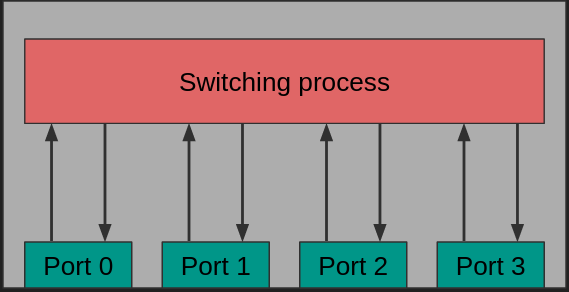
\includegraphics[width=\textwidth]{images/high-level-switch.png}
		\caption{High level overview of a network switch}
	\end{subfigure}
	\hfill
	\begin{subfigure}[b]{0.48\textwidth}
		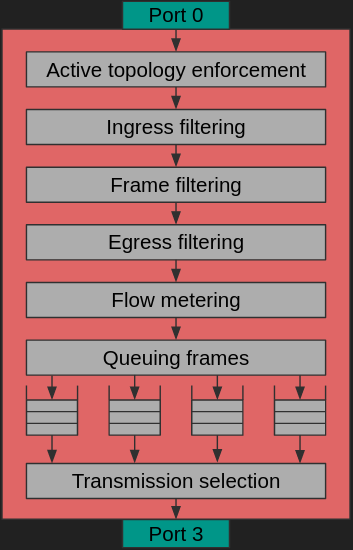
\includegraphics[width=\textwidth]{images/switching-process.png}
		\caption{Internal view of the switching process as specified in clause 8.6 of IEEE 802.1Q-2018}
	\end{subfigure}
	
	\caption{Model of a (TSN) switch showing the steps an Ethernet Frame undergoes between input and output port. Port 0 - Port 4 represent physical ports on the switch used for receiving and transmitting frames}
	\label{fig:switchinternals}
\end{figure} 
To avoid starvation of lower priority streams while still allowing prioritization an alternative \textit{Transmission selection} function has been standardized: IEEE 802.1Qav, known as the Credit Based Shaper (CBS). The Credit Based Shaper sits between a queue and the strict priority scheduler, multiple queues can have a shaper active. Each shaper acts on one specific queue only as depicted in Figure~\ref{fig:cbs}. The Credit Based Shaper limits the maximum bandwidth of a priority class by prohibiting the selection of a new frame when the allocated bandwidth has been consumed. As no frame can be selected from that priority queue, lower priority messages get the chance to be selected next. Whenever the credit of a shaper is zero or higher a frame may be selected by the strict priority scheduler. If the credit is strictly lower than zero no new frames from that queue can be selected for transmission. 
\begin{figure}[htb]
    \centering
    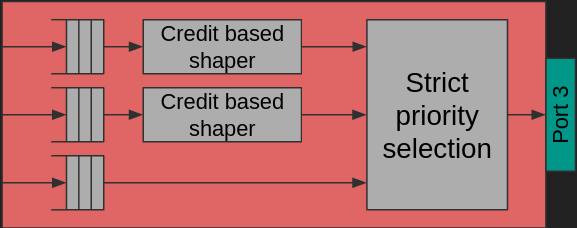
\includegraphics[width=0.6\textwidth]{images/cbs.png}
    \caption{An output port with three queues and the transmission selection implementation consisting of two credit based shapers and a strict priority scheduler}
    \label{fig:cbs}
\end{figure}

Credit of a specific shaper starts of at zero and decreases during the transmission of frames from that queue at a rate called the \textit{sendSlope}. When the credit becomes negative no new frames can be transmitted and the credit increases with a rate called the \textit{idleSlope} until it reaches zero. If the queue contains messages that are being blocked credit rises at the \textit{idleSlope} rate. Positive credit is reset to zero if the queue contains no more frames.

The CBS adds fairness and smooths out traffic bursts by limiting the bandwidth of a specific traffic class, but the total delay over multiple hops can become too large for certain control applications. IEEE 802.1Qbv, sometimes called the Time Aware Shaper (TAS) introduces a Stream Reservation Class CDT for time critical data which specifies a low worst-case latency. The TAS uses a time-division multiple access (TDMA) scheme to define a cyclic network schedule, called the gate control list. The schedule splits the network bandwidth up into time slices and defines which of the Ethernet priorities are allowed to transmit on the network during that time slice. A gate between the queue output and the priority scheduler entry opens or closes to allow or block frames to be selected by the scheduler. If two or more priorities have access to the network at the same time and have messages ready for transmission the normal strict priority scheduler decides the transmission order. An entry in the gate control list defines the state (open/closed) each gate should switch to at a specific time. The Time Aware Shaper can be used to avoid large buffering effects in the switches and removes non-deterministic interruptions by non-real time traffic.

Other shapers exist such as the IEEE 802.1Qcr Asynchronous Traffic Shaper and IEEE 802.1Qch Cyclic Queuing and Forwarding standards. Each working differently and solving a specific problem. The last relevant standards for bounded low latency are the related standards IEEE802.3br and IEEE802.1Qbu which together allow lower priority frames to be preempted during their transmission for the transmission of higher priority frames. The smallest transmittable chunk is still 64 bytes, so the high priority frames will still experience some delay.

\paragraph{Reliable frame transmission} In certain applications it is critical that messages are received without errors in their content. Ethernet protects the frame data by appending a cyclic redundancy check (CRC) and requiring a frame to be dropped when the CRC does not match the received date. Other reasons that a frame is not received can be: switch queues overflowing and hardware failure of connectors or cables. The IEEE 802.1CB standard duplicates frames and sends them over multiple disjoint paths to increase the chance that a frame arrives at the destination. The first duplicate which arrives at the destination and passes the CRC check is considered correct, the remaining frames will be discarded upon reception. If a node does not implement IEEE 802.1CB the closest IEEE 802.1CB aware switch will transparently duplicate/eliminate the frames. In an automotive setting one could imagine two disjoint paths on either side of the vehicle to increase the reliability of the network by placing the redundant paths physically far apart. 

In conclusion there is not one type of TSN network, TSN is a set of different standards trying to solve different problems in one or more ways. Depending on the requirements several TSN standards can be combined to create an Ethernet based network that is capable of reliable, time deterministic and low latency transmission of Ethernet frames. For example the Credit Based Shaper can be used together with the Time Aware Shaper to mix hard, soft and non-real time data in a single network. Which then uses IEEE 802.1CB to reliably deliver the frames over two disjoint paths.

	\clearpage
	\section{Domain}
\label{sec:domain}
\todo{Samenvatting hoofdstuk + structuur (sectie 2.1 ..., 2.2 ...)}
\subsection{Current and future automotive architecture}
\label{sec:architectures}
Modern vehicles are mostly electrically or electronically controlled, ranging from basic functionality such as accelerating and controlling the lights, to more advanced features such as ride height control through a touch screen or autonomous emergency braking. New European legislation will mandate even more of those functions such as an alcohol interlock, driver drowsiness detection, event data recorders and more. Each function is implemented with one or more dedicated electronic control units (ECUs). The ECUs need to communicate together to achieve a certain function and often need to interface with other functions for data or to achieve a certain safety requirement. The current electrical/electronic control architecture is decentralized, and the networks are grouped based on function. For example a drivetrain network or a body control network. In practice vehicles can have more than 100 ECUs~\cite{bandur2021making} and several communication networks. This has several drawbacks, among others: increased communication load on the network, increased costs, increased software complexity, more software variants, higher maintenance costs and reduced reliability~\cite{bandur2021making}. An example of a decentralized function based architecture can be found in Figure~\ref{fig:functional-arch}, the blue rectangles represent ECUs, ECUs that are part of a single function or domain (body control, drivetrain etc) are connected to each other with an automotive network such as LIN or CAN. The functions or domains work together by means of a gateway (red rectangle) which bridges or translates messages to and from the different networks. Sometimes certain ECUs are also connected to more than one network for practical reasons such as the Steering column ECU in the example.

\begin{figure}[htb]
    \centering
    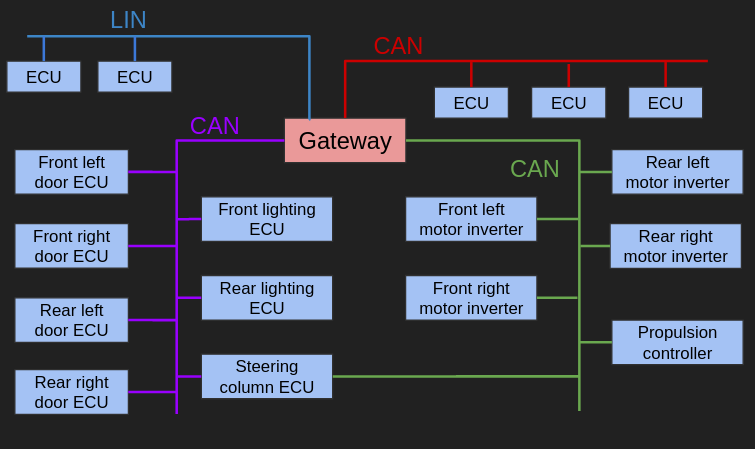
\includegraphics[width=\textwidth]{images/functional-arch.png}
    \caption{Example of an automotive decentralized control architecture}
    \label{fig:functional-arch}
\end{figure}

The rise of advanced driver assistance systems (ADAS) requiring more network bandwidth, extra functions required by European legislation and the aforementioned drawbacks has lead the industry to chose a centralized control architecture with an Ethernet based communication network as the future electrical/electronic architecture, commonly called the zonal architecture~\cite{ashjaei2021time}. Instead of having many small ECUs performing only part of a single function, in the zonal architecture there will be one central ECU responsible for all the control functions and a few larger ECUs, called zone ECUs, which execute the commands of the ECUs. The zone ECUs are strategically placed to handle all functions in the physical neighbourhood of the ECU. To reduce complexity, weight, cost and support ADAS functions, the ECUs are networked through a single high bandwidth, low latency network instead of multiple low bandwidth networks. To ease this transition a zone ECU can act as a bridge for legacy networks used by legacy components in its physical neighbourhood. An example of the zonal architecture with a zone ECU acting as a bridge for a legacy component is shown in Figure~\ref{fig:zonal-arch}

In the new zonal architecture the zone ECU and central controller communicate using a high bandwidth low latency network, automotive Ethernet (single twisted pair physical layer) together with Time Sensitive Networking (TSN) have been chosen as the key networking technologies. The choice for automotive Ethernet is supported by the work of the Time Sensitive Networking (TSN) Task Group of the IEEE 802.1 Working Group, which allow real-time communication over IEEE 802.3 (Ethernet) networks~\cite{klaus2019zonal}. Other relevant factors for choosing automotive Ethernet and TSN are the high bandwidth capabilities relative to traditional networks such as CAN and FlexRay, Internet Protocol (IP) based end-to-end communication support, automotive specific physical layer standards for various data rates, and standardization by the IEEE~\cite{ashjaei2021time}.

\begin{figure}[htb]
    \centering
    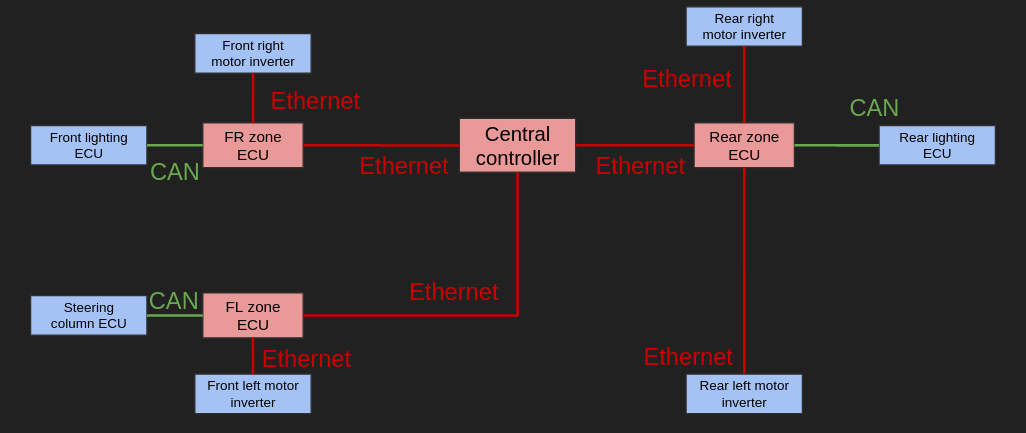
\includegraphics[width=\textwidth]{images/zone-arch.png}
    \caption{Example of an automotive zonal architecture}
    \label{fig:zonal-arch}
\end{figure}

The same vehicle is represented in Figure~\ref{fig:functional-arch} as in Figure~\ref{fig:zonal-arch} but with a decentralized functional architecture and a centralized zonal architecture respectively. The number of ECUs is reduced from 18 to 11 respectively, which is achieved by consolidating ECUs into the zone ECUs, reducing mass. The total number of networks stayed the same, but crucially the physical wiring loom has been simplified in the zonal architecture as there is only a single network going from the back to the front of the vehicle, reducing weight and costs as short wire harnesses can be manufactured automatically.
\subsection{Real-time communication over Ethernet}
\label{sec:real-time-comm}
Some vehicle functions pose strict timing requirements on the architectures and implementations. For example the passenger safety system must always deploy the airbags within a specific time period after a crash. Deploying the airbags too quickly or too late can cause harm to the passengers. Similarly, when the driver presses the brake pedal in an electric vehicle the car should always stop accelerating, apply regenerative braking and illuminate the brake lights within a well-defined period of time. Large or non-deterministic variations in response time are undesirable from a safety and user experience point of view. Such systems with strict timing requirements are called real-time systems and require the timing properties to be bounded and analysable. 

Traditional automotive networks such as LIN, CAN and FlexRay support real-time communication, while IEEE 802.3 Ethernet is not a real-time network. One of the original design philosophies is best-effort transmission of frames~\cite{metcalfe1976ethernet}. Putting the responsibility of dealing with packet loss, duplication, large delays etc. on the communicating processes. This gives good average-case performance to a large group of users in an economically viable way, but sacrifices the real-time property. The switches used in a full-duplex switched Ethernet network introduce a delay in the communication between two nodes. IEEE 802.3 does not specify how a switch should operate, hence in general no guarantee can be made about the queuing and switching delay added to the transmission time by a switch. Additionally, it is reasonable to assume that queuing delays increase as the number of packets passing through a switch increases. Making Ethernet unsuitable for use in a real-time system. 

Several higher level protocols have been proposed to make real-time communication on top of Ethernet possible e.g EtherCAT, PROFINET, TTEthernet and Time Sensitive Networking. Some of these protocols require special network interface cards or switches to operate, or they are not directly interoperable with standard Ethernet, which complicates mixing the network other devices such as a computer using the TCP/IP stack. Time Sensitive Networking (TSN) is a set of standards created by an IEEE Task Group. According to their website\footnote{\url{https://1.ieee802.org/tsn/}, accessed 15 December 2023} their goal is "\textit{... to provide deterministic connectivity through IEEE 802 networks, i.e., guaranteed packet transport with bounded latency, low packet delay variation and low packet loss.}" TSN standards and amendments can be grouped in four categories according to their design goal~\cite{ashjaei2021time}: Timing and synchronization, resource management, bounded low latency and finally high reliability. For each design goal several solutions have been standardized, e.g. several traffic shapers exist which aim for bounded low latency. Each traffic shaper is designed to solve a different problem, but complicating the network design as many choices need to be made during the design phase. Most standards can be combined in the same network e.g, the Credit Based Shaper~\cite{IEEE8021Qav} and Time Aware Shaper~\cite{IEEE8021Qbv}, increasing design complexity. The relevant standards and amendments for the automotive industry have been summarized in Appendix~\ref{appendix:tsn}.
\subsection{Time Sensitive Networking}
\label{sec:tsn}
\todo{Vat dit stuk samen, verhuis details naar sota}
Time Sensitive Networking (TSN) is a set of standards created by an IEEE Task Group. According to their website\footnote{\url{https://1.ieee802.org/tsn/}, accessed 15 December 2023} their goal is "\textit{... to provide deterministic connectivity through IEEE 802 networks, i.e., guaranteed packet transport with bounded latency, low packet delay variation and low packet loss.}" TSN standards and amendments to standards can be grouped in four categories according to their design goal~\cite{ashjaei2021time}: Timing and synchronization, resource management, bounded low latency and finally high reliability. The remainder of this section summarizes and groups the main TSN standards and amendments according to the previously mentioned categories, similar to the work presented in~\cite{ashjaei2021time}.

\paragraph{Globally accurate time base} TSN recognized that having an accurate common notion of time in a network simplifies the design and implementation of real-time systems. A globally accurate and synchronized time base is a central concept in the Time Triggered Architecture~\cite{kopetz2003time} from which TTEthernet was developed. The IEEE 802.1AS-2020~\cite{IEEE8021AS} standard specifies an algorithm called the Best Master Clock Algorithm, for determining the time reference node, called the Grand Master, in the network. The generalized precision time protocol (gPTP) takes care of synchronizing the clocks of all nodes by supplying the Grand Master clock value and taking transmission delay into account. It also provides redundancy in the clock synchronization and Grand Master clock in case of node or link failures.

\paragraph{Network resource management} In cases where real-time network traffic has a dynamic nature, e.g. an audio/video stream that only occurs at specific times in a mixed use network, TSN provides the Stream Reservation Protocol through the IEEE 802.1Qat standard~\cite{IEEE8021Qat}. The Stream Reservation Protocol reserves resources in the bridges between the source and destination nodes of the stream. Resulting in an upfront guarantee that the network meets the streams bandwidth and latency requirement. IEEE 802.1Qcc~\cite{IEEE8021Qcc} extends the Stream Reservation Protocol for more complex networks with different traffic shapers and frame preemption. While the Stream Reservation Protocol uses decentralized registration and reservation, IEEE 802.1Qcc adds centralized configuration management which can coexist with the decentralized stream reservation in the same network.

\paragraph{Deterministic transmission latency} The lack of deterministic transmission latency for Ethernet frames is caused by the network switches, called bridges in the IEEE 802.1Q-2018 standard~\cite{IEEE8021Q}. Time Sensitive Networking leverages the VLAN standard which defines eight priority classes and a strict priority scheduling algorithm. Each physical port of a bridge has a logical input and output port, when a frame enters the input port it undergoes \textit{filtering and metering} before being placed in one of eight queues that are specific for that output port. The frame's priority determines in which queue it is placed. When the output port is free to transmit a frame, the \textit{transmission selection} determines from which queue the next frame will be transmitted. As a basis TSN uses a strict priority scheduler, meaning that the queued message with the highest static priority will always be transmitted first. This can cause starvation of low priority messages.

To avoid starvation whiles still allowing prioritization an alternative \textit{transmission selection} function has been standardized: IEEE 802.1Qav~\cite{IEEE8021Qav}, known as the Credit Based Shaper (CBS). The Credit Based Shaper sits between a queue and the strict priority scheduler. Each shaper acts on one specific queue only as depicted in figure~\ref{fig:cbs}. The Credit Based Shaper limits the maximum bandwidth of a priority class by prohibiting the selection of a new frame when the allocated bandwidth has been consumed. 

The Credit Based Shaper adds fairness and smooths out traffic bursts by limiting the bandwidth of a specific traffic class, but the total delay over multiple hops can become too large for certain control applications. IEEE 802.1Qbv~\cite{IEEE8021Qbv}, called the Time Aware Shaper introduces a Stream Reservation Class \textit{CDT} for time critical data which specifies a low worst-case latency. The Time Aware Shaper uses a time-division multiple access scheme to define a cyclic network schedule called the \textit{gate control list}. The schedule splits the network bandwidth up into time slices and defines which of the Ethernet priorities are allowed to transmit during that time slice. A gate between the queue output and the priority scheduler entry opens or closes to allow or block frames to be selected by the scheduler. The Time Aware Shaper can be used to avoid large buffering effects in the switches and removes non-deterministic interruptions by non-real time traffic.

\begin{figure}[htbp]
    \centering
    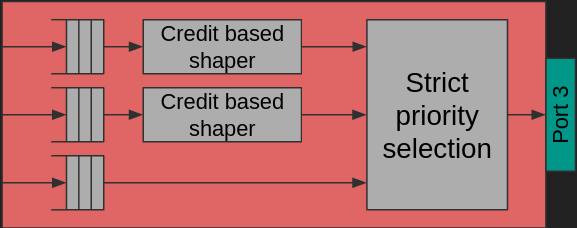
\includegraphics[width=0.6\textwidth]{images/cbs.png}
    \caption{An output port with three queues and the transmission selection implementation consisting of two credit based shapers and a strict priority scheduler}
    \label{fig:cbs}
\end{figure}

Other shapers exist such as the IEEE 802.1Qcr~\cite{IEEE8021Qcr} Asynchronous Traffic Shaper and IEEE 802.1Qch~\cite{IEEE8021Qch} Cyclic Queuing and Forwarding standards. Each working differently and solving a specific problem. The last relevant standards for bounded low latency are the related standards IEEE 802.3br~\cite{IEEE8023br} and IEEE 802.1 Qbu~\cite{IEEE8021Qbu} which together allow lower priority frames to be preempted during their transmission. The smallest transmittable chunk is still 64 bytes, so higher priority frames will still experience some delay. \todo{preemption buffer na de gate, waardoor je preempted bericht alsnog delay kan veroorzaken op een later moment terwijl zijn gate al gesloten is.}

\paragraph{Reliable frame transmission} In certain applications it is critical that messages are received without errors in their content. Ethernet protects the frame data by appending a cyclic redundancy check and requiring a frame to be dropped when the CRC does not match the received data. Other reasons that a frame is not received can be: switch queues overflowing and hardware failure of connectors or cables. The IEEE 802.1CB Frame Replication and Elimination for Reliability~\cite{IEEE8021CB} (FRER) standard duplicates frames and sends them over multiple disjoint paths to increase the chance that a frame arrives at the destination. The first duplicate which arrives at the destination and passes the CRC check is considered correct, the remaining frames will be discarded upon reception. If a node does not implement FRER the closes FRER aware switch will transparently duplicate/eliminate the frames. In an automotive setting one could imagine two disjoint paths on either side of the vehicle to increase the reliability of the network by placing the redundant paths physically far apart.

\paragraph{}In conclusion there is not one type of Time Sensitive Network, TSN is a set of different standards trying to solve different problems in multiple ways. Depending on the requirements several standards can be combined to create an Ethernet based network that is capable of reliable, time deterministic and low latency transmission of Ethernet frames. For example the Credit Based Shaper can be combined with the Time Aware Shaper to mix hard, soft and non-real time traffic in a single network. Combined with Frame Replication and Elimination to reliably and transparently deliver the frames over two disjoint paths.
\subsection{Controller Area Network}
\label{sec:can}
Controller Area Network (CAN) is a networking technology developed by Robert Bosch GMbH in 1983 and later standardized in 1993 as ISO 11898:1993. CAN is an asynchronous serial communication protocol with data rates up to 1 Mbit/s specifically designed for real-time control~\cite{ISO11898} and is organized as a bus architecture. Meaning that each node on the network may transmit a message when it wants, as it is a bus architecture a transmitted message is received by every node on the bus. Carrier Sense Multiple Access/Collision Resolution is used to avoid multiple nodes transmitting concurrently resulting in data errors. The CAN Frame layout together with the physical encoding of the data bits ensures that when two frames are transmitted at the same time the highest priority frame will be delivered. The sender of the lower priority frame detects the collision before data loss occurs and stops transmission, automatically retrying transmission after the higher priority frame is fully delivered. 


	\clearpage
	\section{Problem statement}
\label{sec:problem_statement}
As mentioned in Section~\ref{sec:architectures} the decentralized architecture of current vehicles has several drawbacks such as the low available bandwidth, reliability, cost and software complexity. The centralized zonal architectures aim to solve these problems and can potentially reduce the power usage and weight of the vehicle as there are less ECUs and cables in the vehicle, making the zonal architecture interesting for Lightyear.

Transitioning from a well understood architecture and network to a new architecture and network technology is a difficult and costly task as all prior knowledge, assumptions, best practices and tools become obsolete and need to be developed from scratch. Errors in the architecture which are discovered late in the project may cause the project to be delayed or cancelled, increasing costs significantly. The chance of making a mistake while designing the Time Sensitive Network is significant. As mentioned in Section~\ref{sec:real-time-comm} Time Sensitive Networking is not a single technology but rather a large set of independent standards which can be mixed to achieve a certain design goal. Each independent part of the network can be configured in different ways with different outcomes. For example the schedule of the Time Aware Shaper influences worst-case delay and jitter of messages in the network. But various algorithms exist for generating that schedule, each with a different optimization goal and thus different performance. The physical network layout impacts the performance characteristics as well, since a message that needs to traverse more switches will incur more delay.

Because of the complexity of Time Sensitive Networking a solution that is capable to estimate a network's performance would allow designers to iterate over various network designs. Gaining confidence that the final network will behave as expected and meet the relevant requirements such as message delay and jitter. A strategy to reduce the complexity of the transition between architectures is to reuse the embedded software executing the vehicle functions while only changing the network software. Taking all this into consideration, Lightyear is searching for an answer to the following question:

\begin{quote}
    \emph{What is an effective method for evaluating the effect of various network configurations and architectures based on Time Sensitive Networking when reusing software from a CAN based architecture?}
\end{quote}

\todo{brug naar de specifieke sota, en de research question}
	\clearpage
	\section{State-of-the-art analysis}
\label{sec:sota}
	\clearpage
	\section{Research description}
\label{sec:research_description}
	\clearpage
	\section{Feasibility experiments}
\label{sec:feasibility}
To gauge the feasibility of the proposed graduation project several aspects of the Lightyear 0 were researched and some experiments with tools were performed. This section describes how the research and experiments were performed and the resulting models, descriptions and data of the experiments.

Section~\ref{sec:invehicle} describes the architecture of the Lightyear 0's in-vehicle network, explaining the different types of nodes found in the network, which networks the vehicle has and the connections between component and network. The results were created by both talking to experts on the in-vehicle network, reading documentation and reading code that is deployed on the nodes or used to build the binaries. 
Section~\ref{sec:networktraffic} is an investigation into the data that is generated and consumed by the nodes in the network. The goal is to understand what kinds of dataflows exist in the Lightyear 0 so that the network traffic produced by these flows can be modelled accurately during the graduation project. The execution model of the node types mentioned in Section~\ref{sec:invehicle} is described as well to make the dataflow model more accurate. Some scripts have been developed to partially retrieve and generate overviews of the dataflow from the program code. This section is a result of inspecting the build-system and the code that is deployed on the network nodes, followed by a review by the architects and lead software developers of the system.

Lastly in Section~\ref{sec:omnetpp} two experiments performed with the Discrete Event Simulator Omnet++ are explained. The first experiment is a re-implementation of an exercise performed during the \textit{Quantitative Evaluation of Embedded Systems} course which was originally executed in Matlab. The goal is to learn the basics of the simulation framework and validate its ability to perform experiments involving random processes. The second experiment sketches a model of periodic dataflow between software components as found in the Lightyear 0.

\subsection{The in-vehicle network}
\label{sec:invehicle}
The Lightyear 0's in-vehicle network is based on a decentralized domain architecture, with CAN and LIN as the main network technologies with Ethernet being used for non-real time applications. Meaning that networked components pertaining to the same function or domain (body control, powertrain etc.) are grouped together in a network. The networks are linked together using a central gateway who is responsible for bridging necessary data between networks. For example information about the motor power might be required in the Battery Management System, Propulsion Controller and Media Controller. But for various reasons these controllers might not all be connected to the same network, so the motor power information needs to be forwarded on the relevant networks.

At the core of the embedded system are three ECUs named the Central Gateway, Vehicle Control Unit and Safety Control Unit. The Safety Control Unit contains two heterogeneous cores, that both have access to the connected CAN busses. Each ECU has a real-time operating system (RTOS) with a rate monotonic preemptive scheduler and can be connected up to four CAN busses and two LIN busses. The software on these ECUs is developed by Lightyear and thus the functionality of an ECU is not fixed or prescribed by a vendor. As the functionality is not fixed we will call these ECUs \textit{programmable end nodes} for modelling purposes.

The other nodes in the network have a fixed function, some of them are developed by Lightyear such as motor inverters and solar converters, while others are developed by third parties. Some of these nodes can be configured by the user to tune the behaviour, while others are completely fixed. In some cases the parameters that can be changed are related to the network behaviour e.g., changing the CAN identifiers of certain messages. For ease of modelling we call these fixed function nodes \textit{parametrizable end nodes}, even if a node is completely fixed and cannot be configured. The inner workings of parametrizable end nodes varies and is often unknown in case of third party components. Fortunately the only necessary knowledge for an accurate network simulation is the external behaviour. Because parametrizable end nodes must be integrated, a precise specification of the network traffic generated and consumed by the end node is available and can be used for modelling purposes.

Three special cases of parametrizable end nodes are worth mentioning, the motor inverters (inverter), the media ECU and the telematics control unit. The motor inverters and media ECU have both a CAN interface and Ethernet interface. The telematics control unit has a CAN interface, Ethernet interface and a wireless modem, giving access to the internet which is shared with the media ECU so that applications such as navigation can use online services.

Table~\ref{tab:networks} gives an overview of all the networks in the car and which nodes are connected to which bus. For brevity a subset of the \textit{parametrizable end nodes} is enumerated, it can be assumed that each bus has several extra nodes connected. Information of the not mentioned nodes is available but simply left out for space reasons. The two LIN busses, LIN A and LIN B, each connect to the Central Gateway which acts as the master in the LIN networks. The slave nodes are third party off the shelf components and can be classified as \textit{parametrizable end nodes}. The same information is represented in diagram form in Figure~\ref{fig:networkoverview}.

Finally, there are components in the vehicle that generate or consume data but are not seen as a networked component in the "traditional" sense. Examples of such components are speakers, which consume audio data, rearview cameras which produce image data, instrument cluster displays which consume video/graphical data. Further investigation is necessary to determine how many of these nodes exist, how they are connected and how they should be modelled from a networking perspective.

\begin{table}[htb]
    \centering
    \resizebox{\textwidth}{!}{%
    \begin{tabular}{@{}lllllllllllllllllll@{}}
                                & \multicolumn{10}{c}{Controller Area Network} & \multicolumn{2}{c|}{LIN} & \multicolumn{5}{c}{Ethernet} & \multicolumn{1}{c}{Other} \\* \cmidrule(lr){2-11} \cmidrule(r){12-13} \cmidrule(r){14-18} \cmidrule(r){19-19}
    Node name                & \multicolumn{1}{R{2.5cm}}{Driver support} & \multicolumn{1}{R{2cm}}{Drivetrain} & \multicolumn{1}{R{2cm}}{Energy\\ management} & \multicolumn{1}{R{2cm}}{HVBS} & \multicolumn{1}{R{2cm}}{Powertrain} & \multicolumn{1}{R{2cm}}{Solar} & \multicolumn{1}{R{2cm}}{Surrounding\\ sense} & \multicolumn{1}{R{2cm}}{Telematics} & \multicolumn{1}{R{2cm}}{Vehicle} & \multicolumn{1}{R{2cm}}{Vehicle 2} & \multicolumn{1}{R{2cm}}{LIN A} & \multicolumn{1}{R{2cm}|}{LIN B} & \multicolumn{1}{R{2cm}}{Media} & \multicolumn{1}{R{2cm}}{Inverter FL} & \multicolumn{1}{R{2cm}}{Inverter FR} & \multicolumn{1}{R{2cm}}{Inverter RL} & \multicolumn{1}{R{2cm}}{Inverter RR} & \multicolumn{1}{R{2cm}}{Others}   \\*\cmidrule(r){1-1} \cmidrule(r){2-11}\cmidrule(r){12-13} \cmidrule(r){14-18} \cmidrule(r){19-19}
    Vehicle Control Unit     & X &   &   &   &   & X & X &   & X &   &   & \multicolumn{1}{c|}{}  &   &   &   &   &   &   \\
    Central Gateway          &   &   &   &   & X &   &   & X & X & X & X & \multicolumn{1}{c|}{X} &   &   &   &   &   &   \\
    Safety Control Unit      &   & X & X & X & X &   &   &   &   &   &   & \multicolumn{1}{c|}{}  &   &   &   &   &   &   \\
    Steering Column Module   & X &   &   &   &   &   &   &   &   &   &   & \multicolumn{1}{c|}{}  &   &   &   &   &   &   \\
    Inverter FL              &   & X &   &   &   &   &   &   &   &   &   & \multicolumn{1}{c|}{}  &   & X &   &   &   &   \\
    Inverter FR              &   & X &   &   &   &   &   &   &   &   &   & \multicolumn{1}{c|}{}  &   &   & X &   &   &   \\
    Inverter RL              &   & X &   &   &   &   &   &   &   &   &   & \multicolumn{1}{c|}{}  &   &   &   & X &   &   \\
    Inverter RR              &   & X &   &   &   &   &   &   &   &   &   & \multicolumn{1}{c|}{}  &   &   &   &   & X &   \\
    High Voltage Battery     &   &   &   & X &   &   &   &   &   &   &   & \multicolumn{1}{c|}{}  &   &   &   &   &   &   \\
    On-board charger         &   &   & X &   &   &   &   &   &   &   &   & \multicolumn{1}{c|}{}  &   &   &   &   &   &   \\
    Media ECU                &   &   &   &   & X &   &   &   &   &   &   & \multicolumn{1}{c|}{}  & X &   &   &   &   & X \\
    Steering Angle Sensor    &   &   &   &   & X &   &   &   &   &   &   & \multicolumn{1}{c|}{}  &   &   &   &   &   &   \\
    Dual String Controller 1 &   &   &   &   &   & X &   &   &   &   &   & \multicolumn{1}{c|}{}  &   &   &   &   &   &   \\
    Camera Monitoring System &   &   &   &   &   &   & X &   &   &   &   & \multicolumn{1}{c|}{}  &   &   &   &   &   &   \\
    Parking Sensor System    &   &   &   &   &   &   & X &   &   &   &   & \multicolumn{1}{c|}{}  &   &   &   &   &   &   \\
    Telematics Control Unit  &   &   &   &   &   &   &   & X &   &   &   & \multicolumn{1}{c|}{}  & X &   &   &   &   &   \\
    Window Wiper             &   &   &   &   &   &   &   &   & X &   &   & \multicolumn{1}{c|}{}  &   &   &   &   &   &   \\
    RC Compressor            &   &   &   &   &   &   &   &   & X &   &   & \multicolumn{1}{c|}{}  &   &   &   &   &   &   \\
    Tailgate Latch           &   &   &   &   &   &   &   &   &   & X &   & \multicolumn{1}{c|}{}  &   &   &   &   &   &   \\
    Rain light sensor        &   &   &   &   &   &   &   &   &   &   & X & \multicolumn{1}{c|}{}  &   &   &   &   &   &   \\
    Air flap actuator        &   &   &   &   &   &   &   &   &   &   &   & \multicolumn{1}{c|}{X} &   &   &   &   &   &   \\
    Speaker Left             &   &   &   &   &   &   &   &   &   &   &   & \multicolumn{1}{c|}{}  &   &   &   &   &   & X \\
    Display                  &   &   &   &   &   &   &   &   &   &   &   & \multicolumn{1}{c|}{}  &   &   &   &   &   & X \\
    Rearview camera          &   &   &   &   &   &   &   &   &   &   &   & \multicolumn{1}{c|}{}  &   &   &   &   &   & X \\
\end{tabular}%
}
\caption{Partial overview of in-vehicle networks and nodes}
\label{tab:networks}
\end{table}

\begin{figure}[htb]
    \centering
\begin{tikzpicture}[
    programmablenode/.style={rectangle, draw=lightblue, fill=lightblue},
    parametrizablenode/.style={rectangle, draw=orange, fill=orange},
    canbus/.style={rectangle, fill=mint},
    linbus/.style={rectangle, fill=pink},
    ethernet/.style={rectangle, fill=olive},
    other/.style={rectangle, fill=palegrey},
]
    % Nodes & Networks
    \node[programmablenode] (SCU) {Safety Control Unit};
    \node[canbus] (PT) [above=of SCU] {Powertrain};
    \node[programmablenode] (CGW) [above=of PT]{Central Gateway};
    \node[canbus] (VEHICLE) [above=of CGW] {Vehicle};
    \node[programmablenode] (VCU) [above=of VEHICLE]{Vehicle Control Unit};
    \draw[-] (SCU.north) -- (PT.south);
    \draw[-] (CGW.south) -- (PT.north);
    % Driver support
    \node[canbus] (DS) [right= of VCU] {Driver Support};
    \node[parametrizablenode] (SCM) [above=of DS] {Steering Column Module};
    \draw[-] (DS.west) -- (VCU.east);
    \draw[-] (DS.north) -- (SCM.south);
    % Drivetrain
    \node[canbus] (DT) [below= of SCU] {Drivetrain};  
    \node[parametrizablenode] (INVFL) [below left=of DT]{Inverter FL};
    \node[parametrizablenode] (INVFR) [below =of INVFL]{Inverter FR};
    \node[parametrizablenode] (INVRL) at (DT|-INVFL){Inverter RL};
    \node[parametrizablenode] (INVRR) at (DS|-INVFL){Inverter RR};
    \draw[-] (SCU.south) -- (DT.north);
    \draw[-] (INVFL.north) -- (DT.west);
    \draw[-] (DT.south west) -- (INVFR.north east);
    \draw[-] (DT.south) -- (INVRL.north);
    \draw[-] (DT.south east) -- (INVRR.north west);
    % Energy Management
    \node[canbus] (EM) at (DS|-SCU) {Energy Managment};
    \node[parametrizablenode] (OBC) [below= of EM] {On-board charger};
    \draw[-] (EM.west) -- (SCU.east);
    \draw[-] (EM.south) -- (OBC.north);
    % Powertrain
    \node[parametrizablenode] (MEDIA) [left= of SCU] {Media ECU};
    \node[parametrizablenode] (SAS) at (DS|-PT) {Steering angle sensor};
    \draw[-] (MEDIA.north) -- (PT.west);
    \draw[-] (SAS.west) -- (PT.east);
    % Surounding Sense
    \node[canbus] (SS) [above= of VCU] {Surounding Sense};
    \node[parametrizablenode] (PSS) [above right=of SS] {Parking Sensor System};
    \node[parametrizablenode] (CMS) [above=of SS] {Camera Monitoring System};
    \draw[-] (VCU.north) -- (SS.south);
    \draw[-] (SS.north) -- (CMS.south);
    \draw[-] (SS.north east) -- (PSS.south west);
    % Solar
    \node[canbus] (SOLAR) [left=of SS] {Solar};
    \node[parametrizablenode] (DSC) [left=of CMS] {Dual String Converter 1};
    \draw[-] (SOLAR.south east) -- (VCU.north west);
    \draw[-] (DSC.south) -- (SOLAR.north);
    % Telematics
    \node[canbus] (TELE) [left=of PT] {Telematics};
    \node[parametrizablenode] (TCU) [left=of TELE] {Telematics Control Unit};
    \node[ethernet] (MEDIAETH) at(TCU|-MEDIA) {Media Ethernet};
    \draw[-] (CGW.south west) -- (TELE.north east);
    \draw[-] (TELE.west) -- (TCU.east);
    \draw[-] (MEDIAETH.north) -- (TCU.south);
    \draw[-] (MEDIAETH.east) -- (MEDIA.west);
    % HVBS
    \node[canbus] (HVBS) [below left= of SCU] {HVBS};
    \node[parametrizablenode] (BAT) at(MEDIAETH|-HVBS) {High Voltage Battery};
    \draw[-] (HVBS.north east) -- (SCU.south west);
    \draw[-] (HVBS.west) -- (BAT.east);
    % Vehicle
    \node[parametrizablenode] (WIP) at (DS|-VEHICLE) {Window Wiper};
    \node[parametrizablenode] (COMP) [below=of WIP] {RC Compressor};
    \draw[-] (CGW.north) -- (VEHICLE.south);
    \draw[-] (VEHICLE.north) -- (VCU.south);
    \draw[-] (VEHICLE.east) -- (WIP.west);
    \draw[-] (VEHICLE.south east) -- (COMP.west);
    % Vehicle2
    \node[canbus] (VEHICLE2) [left=of VCU] {Vehicle 2};
    \node[parametrizablenode] (LATCH) at (DSC|-SOLAR) {Tailgate Latch};
    \draw[-] (VCU.west) -- (VEHICLE2.east);
    \draw[-] (VEHICLE2.north west) -- (LATCH.south);
    %INVerter Ethernet
    \node[ethernet] (ETHFL) at(MEDIAETH|-INVFL) {Inverter FL};
    \draw[-] (INVFL.west) -- (ETHFL.east);
    \node[ethernet] (ETHFR) at(MEDIAETH|-INVFR) {Inverter FR};
    \draw[-] (INVFR.west) -- (ETHFR.east);
    \node[ethernet] (ETHRL) at(INVRL|-INVFR) {Inverter RL};
    \draw[-] (INVRL.south) -- (ETHRL.north);
    \node[ethernet] (ETHRR) at(INVRR|-INVFR) {Inverter RR};
    \draw[-] (INVRR.south) -- (ETHRR.north);
    %LIN busses
    \node[linbus] (LINA) at(MEDIA|-VEHICLE) {LINA};
    \node[parametrizablenode] (RAIN) at(TCU|-LINA) {Rain light sensor};
    \draw[-] (RAIN.east) -- (LINA.west);
    \draw[-] (LINA.east) -- (CGW.north west);
    \node[linbus] (LINB) at(MEDIA|-CGW) {LINB};
    \node[parametrizablenode] (AIR) at (TCU|-LINB) {Air flap actuator};
    \draw[-] (AIR.east) -- (LINB.west);
    \draw[-] (LINB.east) -- (CGW.west);
    %Legend
    \filldraw[palegrey, thick] (-8.3,10.3) rectangle (6.0, 13);
    \node[programmablenode] (PROG) [align=center] at (TCU|- 50,11){Programmable\\ end node};
    \node[parametrizablenode] (PARA) [right=of PROG, align=center] {Parametrizable\\ end node};
    \node[canbus] (CAN) [right=of PARA] {CAN bus};
    \node[linbus] (LIN) [right=of CAN] {LIN bus};
    \node[ethernet] (ETH) [right=of LIN, align=center] {Ethernet\\ network};
    \node[] (Legend) at (-1.1,12.5) {Legend};
    
\end{tikzpicture}
\caption{Partial block diagram of the in-vehicle networks and nodes}
\label{fig:networkoverview}
\end{figure}
\clearpage
\subsection{Network traffic}
\label{sec:networktraffic}
\paragraph{Programmable end node}
The software for the \textit{programmable end nodes} implementing the required functions is decoupled from the physical node it is deployed on. From a programmers point of view the software is split up un several logical nodes. Each node is responsible for implementing a certain related set of functions, examples of logical nodes are: the \textit{Braking System Manager} or the \textit{Lighting Manager}. The logical nodes consist of one or more runnables, the runnable is the smallest software component that is subject to scheduling by the RTOS. This allows to split a logical node in several runnables which can be scheduled independently or deployed on different physical nodes. Runnables communicate with each other through signals, a signal represents a sample of some system state variable. These system state variables can represent a physical value or an abstract value. For example as displayed in Figure~\ref{fig:logical}, \textit{brake pedal applied} could be a signal generated by a runnable of the \textit{Braking System Manager}, describing whether the brake pedal is being pressed by the driver. A \textit{Lighting Manager} runnable could consume the \textit{brake pedal applied} signal to determine whether the brake lights should be lit. A signal is produced by a single runnable, but can be consumed by multiple runnables. For each logical node a set of deployment files describe which runnables exist, which signals are consumed and produced by each runnable, at what rate the runnables are scheduled and on which \textit{programmable end nodes} they are deployed.

\begin{figure}[htbp]
    \centering
    \resizebox{0.95\textwidth}{!}{%
        \tikzfig{logical_example}
    }
 \caption{Example of two logical components consisting of several runnables communicating through signals}
\label{fig:logical}
\end{figure}

The deployment files are used when building binaries for the \textit{programmable end nodes} to automatically generate code to bridge the required signals between the runnables. First let's consider a pair of runnables consuming/producing the same signal that are deployed on the same \textit{programmable end node}. So one runnable generates a signal while the other is a consumer of that signal. Because the runnables are deployed on the same \textit{programmable end nodes} there is no network traffic necessary. In this case the signal can be thought of as being implemented as a global variable residing in the \textit{programmable end nodes} memory which can be accessed in a thread-safe way by both runnables.

If the producing and consuming runnables are deployed on different \textit{programmable end nodes} which are directly connected to each other e.g, the Vehicle Control Unit and the Central Gateway, the signal has to be transmitted on the network connecting them. In this case the signal is transmitted to the receiving node over CAN at a fixed rate. For efficiency reasons signals that have the same \textit{programmable end node} as destination are packed in the same CAN message. See Figure~\ref{fig:deployment} for an example deployment of two logical nodes, a \textit{Vehicle Power Controller} consisting of two runnables, and the \textit{Exterior Lighting} logical consisting of a single runnable. And two signals \textit{active\_gear} and \textit{power\_mode} that are produced and consumed by the runnables.

\begin{figure}[htbp]
    \centering
    \resizebox{\textwidth}{!}{%
        \tikzfig{deployment_example}
    }
 \caption{Example of two logical components consisting of several runnables communicating through signals}
\label{fig:deployment}
\end{figure}

The last case is when a producing and consuming runnable are deployed on different \textit{programmable end nodes} which are not directly connected to each other e.g, the Vehicle Control Unit and Safety Control Unit. In this case the message has to be bridged across two networks by the Central Gateway. For modelling purposes one can think of having two runnables in the Central Gateway responsible for bridging the data from node A to B. The first being the \textit{gateway\_receive} runnable, which consumes signals from node A. The second being the \textit{gateway\_transmit} runnable, which produces signals for the runnables running on \textit{programmable end node} B, forwarding the consumed signal from the \textit{gateway\_receive} runnable.

Because signals can be consumed by multiple runnables, combinations of the cases mentioned above are possible for a single signal. For example a signal can be consumed by a runnable deployed on the same \textit{programmable end node} and by a runnable on a node without direct CAN connection, requiring bridging by the Central Gateway.

Because the deployment can change as development progresses but also because a deployment is specific to a vehicle type we want to create a description of the data flow on the logical level. This description can be used as an input for generating several deployments whose performance can be evaluated using simulation. The data flow description is specific for a vehicle as it is influenced by the chosen architecture and the feature set. It can serve as a benchmark for a type of vehicle with a known feature set. The data flow description can be adapted to match vehicles with different architectures and feature sets. 

From the deployment files we can generate an interface overview of the \textit{programmable end node} software i.e, a list detailing the source runnable of a signal and which runnables consume that signal together with several other signal attributes such as the data type (integer, enumerate, etc.). This gives us a part of the logical architecture data flow. As described earlier the runnables executing on the \textit{programmable end nodes} generate network traffic when signals are shared between runnables on separate nodes. The deployment files contain the mapping of runnable to \textit{programmable end node}, together with the logical data flow it is possible to generate an interface overview detailing the source and destination in the physical architecture for each signal. A script has been created to generate such interface overviews both in tabular (machine readable) form, for further processing by to be created software as in graphical form to aid in debugging issues in the vehicle. Table~\ref{tab:interface_overview} shows the tabular output of the script for two signals in the Lightyear 0, the \textit{active\_gear} signal is produced by the \textit{Vehicle Power Controler} logical component in the primary core of the \textit{Safety Control Unit} ECU, it is consumed by three other logicals executing in the \textit{Safety Control Unit} primary core and by four logicals executing in two different \textit{programmable end nodes}. Figure~\ref{fig:interface_overview} displays the same information in a directed graph. The circular nodes represent the signal while the rectangular nodes represent the runnable consuming/producing the signal. An edge originating in the signal node and ending in a runnable node represents that the signal is consumed by the destination runnable. An edge originating in a runnable node and ending in the signal node represents that the runnable produces the signal.

\begin{table}[htbp]
    \centering
    \resizebox{\textwidth}{!}{%
    \begin{tabular}{@{}llllll@{}}
    \toprule
    signal name  & source physical  & source logical           & destination physical   & destination logical         & data type        \\ \midrule
    active\_gear & scu\_primary     & Vehicle Power Controller & scu\_primary           & Braking System Manager      & int16\_t         \\
    power\_mode  & central\_gateway & VPC Gateway              & scu\_primary           & Vehicle Power Controller    & i\_psm\_state\_t \\
    power\_mode  & central\_gateway & VPC Gateway              & scu\_primary           & Energy Storage Controller   & i\_psm\_state\_t \\
    active\_gear & scu\_primary     & Vehicle Power Controller & scu\_primary           & Gear Selector Manager       & int16\_t         \\
    active\_gear & scu\_primary     & Vehicle Power Controller & scu\_primary           & Safety Supervisor Core      & int16\_t         \\
    power\_mode  & central\_gateway & VPC Gateway              & scu\_primary           & Safety Supervisor Core      & i\_psm\_state\_t \\
    active\_gear & scu\_primary     & Vehicle Power Controller & central\_gateway       & Authentication Manager      & int16\_t         \\
    active\_gear & scu\_primary     & Vehicle Power Controller & central\_gateway       & Media ECU Interface Manager & int16\_t         \\
    active\_gear & scu\_primary     & Vehicle Power Controller & central\_gateway       & Lighting Manager            & int16\_t         \\
    active\_gear & scu\_primary     & Vehicle Power Controller & vehicle\_control\_unit & Driver Controls Manager     & int16\_t         \\
    power\_mode  & central\_gateway & VPC Gateway              & vehicle\_control\_unit & Solar Controller            & i\_psm\_state\_t \\
    power\_mode  & central\_gateway & VPC Gateway              & vehicle\_control\_unit & VPC vcu                     & i\_psm\_state\_t \\ \bottomrule
    \end{tabular}%
    }
    \caption{Interface overview for \textit{power\_mode} and \textit{active\_gear} signals}
    \label{tab:interface_overview}
    \end{table}

\begin{figure}[htbp]
    \centering
    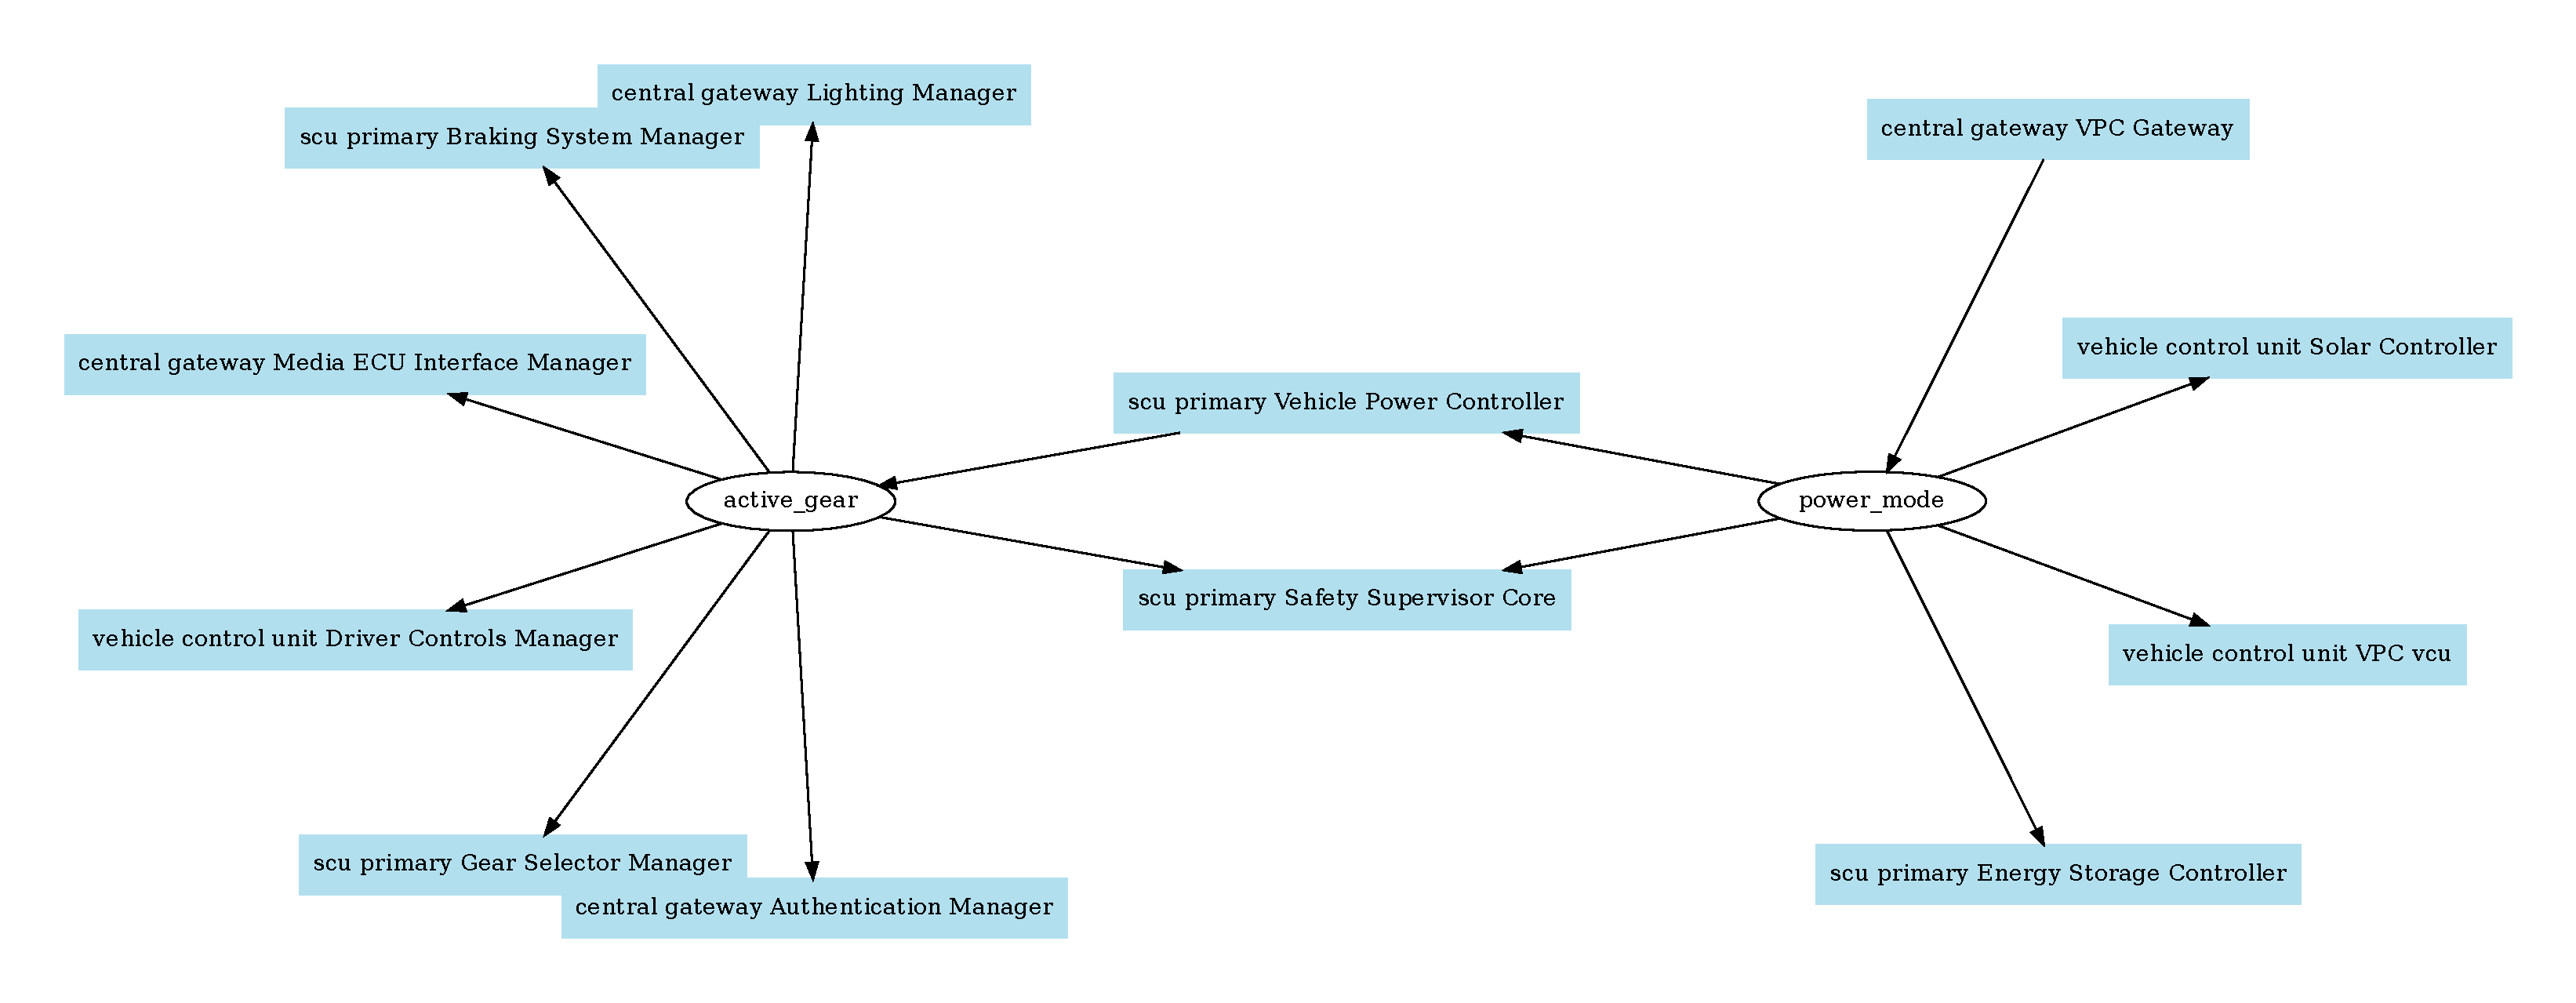
\includegraphics[width=\textwidth]{images/interface_overview.pdf}
    \caption{Interface overview for two signals in graphical form}
    \label{fig:interface_overview}
\end{figure}

\paragraph{Parametrizable end nodes}
The network traffic to and from \textit{parametrizable end nodes} is described in special deployment files called DBC files for CAN networks and LDF files for LIN networks. These are industry standards describing the messages that can be found on a network. For each message the content is described in terms of signals and how the raw bytes transmitted on the network map to a signal value. For example a signal \textit{brake pedal position} describing a numerical value has a certain data type (single precision floating point, 16-bit signed integer, 32-bit unsigned integer), but the numerical value can be also scaled and offset to represent the real value. The DBC and LDF standards describe how a set of received bytes can be reinterpreted as the original signal and how a measured value must be transformed in a set of bytes to transmit. 

In order to get the data flow to and from \textit{parametrizable end nodes} the LDF and DBC files are necessary as they describe which signals are communicated. Unfortunately these files do not always describe the source and destination of a signal, nor do they accurately describe the transmission rate, nor is it known which runnable from the \textit{programmable end nodes} consumes/produces the signal. This information is not available in a central and easily machine-readable format. A possible solution for partially retrieving this information is through static analysis of the \textit{programmable end node} software. The reception and transmission of the signals using the CAN and LIN busses happens by using a specific set of interfaces provided by the RTOS. By analysing call graphs of these interfaces the missing information could be retrieved. Some inaccuracies in the exact transmission rate of the signals might be introduced, but that is an acceptable risk given that we are using the data flow description as an input for simulating and evaluating various network configurations. A second solution would be to assume that each node on the bus consumes the transmitted data at exactly the rate at which it is transmitted. This would solve the lack of source and destination information but still misses the transmission rate. Additionally, it would introduce inaccuracies that could make the data flow description too pessimistic.

\paragraph{Aperiodic and non-real time data}
The description of dataflow by the various nodes so far serves as input/output of the various control applications in the vehicle e.g, cruise control or battery management, this type of traffic is (mostly) periodic and has a defined transmission rate. Data that is unrelated to the control systems is served on the same networks. For example applications such as software updates, remote diagnostics, logging of crucial signals all generate data that requires bandwidth on the network to reach the appropriate destination. To accommodate the complex requirements of these applications a transport layer is used to allow transmitting data packets with a data size that is larger than the maximum data size of a CAN frame. The chosen protocol is ISO~15765, known as ISO-TP, which acts as the network and transport layer in the OSI model.

The Telematics Control Unit (TCU) regularly checks if software updates are available, when an update is initiated the TCU transmits the update using ISO-TP to the end node that is updated. Because the TCU only has a direct CAN connection with the Central Gateway the update stream must be bridged by the Central Gateway to the correct CAN bus. When the to be updated end node has no direct connection with the Central Gateway, such as the inverters (Table~\ref{tab:networks}), the stream must be bridged again in this example by the Safety Control Unit. Similarly, logging of crucial signals occurs in an online database. The data is collected by the \textit{programmable end nodes} and transmitted to the TCU using ISO-TP. 

When a vehicle has to be serviced a technician can connect to the diagnostics port and run diagnostics using the industry standard ISO~14229 - Unified Diagnostic Services (UDS). UDS is a communication protocol specifically designed for diagnostics in vehicles. It allows technicians to read error codes of all the nodes in the network, perform tests and configure certain parameters. UDS uses ISO-TP as the transport layer, as the diagnostics port is connected to the Central Gateway bridging of the UDS messages occurs similarly to the software update stream when an end node is not directly connected to the Central Gateway.

Further investigation is necessary to understand which nodes generate aperiodic and non-real time data and what the underlying processes are that trigger this data to be transmitted. It is likely that certain dataflows only occur in specific use-cases, for example the diagnostics data will (probably) only occur when a service technician connects hardware to the diagnostics port and reads the status of the vehicle hardware. While other data streams can occur regularly during normal use of the vehicle, such as logging of specific signals in the cloud.

As shown previously the vehicle has several Ethernet networks. The inverters contain many internal signals which need to be sampled or change at high speeds (in the kHz range) to operate correctly e.g., current and voltage measurements. This is too much data to transmit over a CAN bus and can be irrelevant for other applications connected to the CAN bus. Hence, this data is transmitted over the Ethernet network such that during development and testing accurate information is available. The inverter Ethernet interfaces are strictly used for testing and debugging purposes only, nevertheless this is an interesting use case to consider during the design of a TSN based in-vehicle network.
\clearpage
\subsection{Discrete Event Simulation in \omnet}
\label{sec:omnetpp}
Since most relevant literature we wish to build upon uses \omnet as their discrete event simulation framework some experiments were performed. The first goal of the experiments is to create a working installation of \omnet and create a development environment in which the proposed solution can be developed. The second goal is to get acquainted with the modelling language and framework. Lastly the experiments validate that the framework is suitable for performing experiments involving random processes.

After installing \omnet and creating a development environment the \omnet tutorial~\cite{omnettutorial} was followed. This tutorial consists of 18 exercises showing the different aspects of the NED language and framework. To further study the framework and asses the suitability of \omnet for experiments of random processes an assignment from the Embedded Systems course 2IMN25 - Quantitative Evaluation of Embedded Systems is performed again. During the course a theoretical model for the expected steady-state distribution of the number of items in an $M/M/1/K$ queue was made, let $x$ be the number of items in the system, $k$ the maximum number of items in the system, $\lambda$ the arrival rate of items and $\mu$ the service rate of the items, then for $0 \leq x\leq k$ the probability of finding $x$ items in the system is described using Equation~\ref{eq:mm1k}. 
\begin{equation}
    \label{eq:mm1k}
p_\infty (x) = \left(\frac{\lambda}{\mu}\right)^x\cdot\frac{1-\frac{\lambda}{\mu}}{1-\left(\frac{\lambda}{\mu}\right)^{k+1}}
\end{equation}

A model of an $M/M/1/K$ queueing system was made in \omnet which is visualized in Figure~\ref{fig:mm1k_sim}. The system consists of an \textit{entityGenerator} which creates items with an intergeneration time that is drawn from an exponential distribution with a configurable rate $\lambda$. The generated items are then stored in a \textit{queue} of configurable size $K$. The \textit{sink} component takes an item from the \textit{queue} and takes execution time to handle the item before discarding it. The execution time is also drawn from an exponential distribution with a configurable rate $\mu$. An experiment is set up in which we log the queue occupancy in the steady state, \omnet is configured to automatically log the queue occupancy, run a simulation for 800000 s of simulated time and discard the data from the warm-up period of 300000 seconds of simulated time. Because the queue occupancy data points from a single simulation are not independent of each other \omnet is configured to repeat the simulation 50 times with different seed values for the random distributions.

\begin{figure}[htbp]
    \centering
    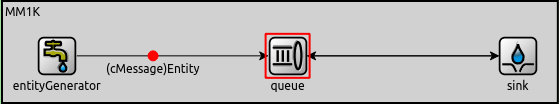
\includegraphics[width=\textwidth]{images/MM1K_sim.png}
    \caption{Visual view of an MM1K queue model in \omnet}
    \label{fig:mm1k_sim}
\end{figure}

The resulting data points are analysed with a python script in which we calculate the probability to find a certain queue occupancy in the simulation, with a 95\% confidence interval. The result of the simulation as well as the theoretical pdf are shown in Figure~\ref{fig:mm1k_sim}. The theoretical pdf falls inside the 95\% confidence interval for every queue occupancy, from this we conclude that the framework is able to properly simulate a random process.

\begin{figure}[htbp]
    \centering
    \includegraphics[width=\textwidth]{images/MM1k_analysis.png}
    \caption{Comparison of MM1K queue occupancy between simulation and theoretical analysis}
    \label{fig:MM1K_analysis}
\end{figure}
\todo{Pitfall in \omnet is manual memory management of events, can cause memory leaks}
\todo{write about logical modelling}

\begin{figure}[htb]
    \centering
    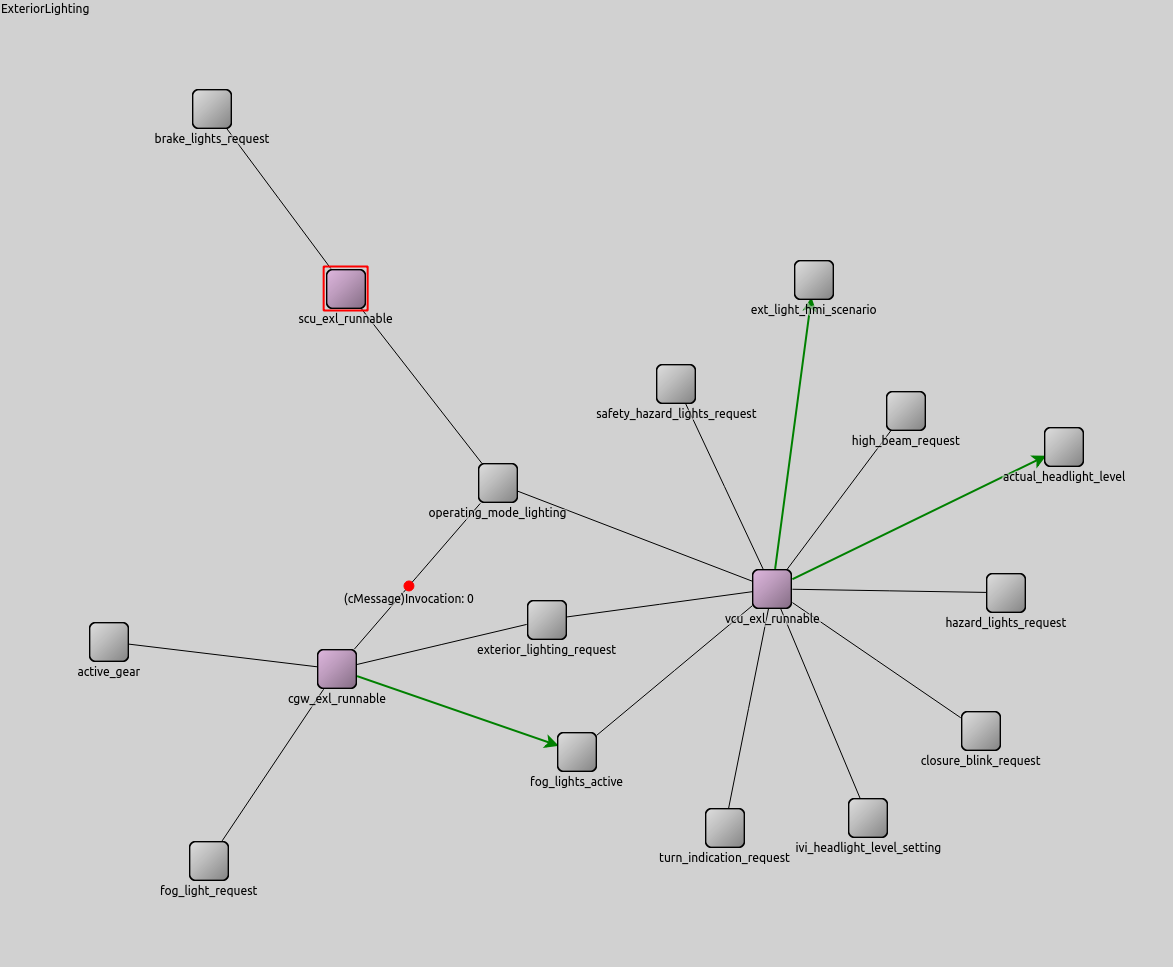
\includegraphics[width=\textwidth]{images/logical_sim.png}
    \caption{Modelling signal transmission of the logical architecture in \omnet}
    \label{fig:logical_sim}
\end{figure}

\newpage
	\clearpage
	\section{Planning}
\label{sec:planning}
The project has a duration of 6 months i.e. 26 weeks and starts after the approval of the preparation phase, of which this document is the result. A high level planning for the project is detailed below.

\begin{table}[htb]
	\centering
	\begin{tabularx}{\textwidth}{@{}lX@{}}
		\toprule
		\textbf{Week} 	& \textbf{Task} \\ \midrule
						& \textbf{Creation of machine-readable network and dataflow benchmark} \\
		1 - 2			& Extract logical \& physical architecture \& periodic dataflow of runnables.  \\
		3 - 5			& Extract logical \& physical architecture \& periodic dataflow to and from parametrizable end nodes.\\\midrule
						& \textbf{Simulation environment} \\
		6 - 7			& Research network requirements \& driving performance indicators \\
		8 				& Investigate which network standards and configurations exist, are relevant and are implemented in \omnet. \\
		9 - 12			& Create model of runnables, programmable end nodes and inter-runnable periodic dataflow for use in an \omnet TSN simulation.\\
		13 - 15 		& Create model of parametrizable end nodes and related periodic dataflow for use in an \omnet TSN simulation \\ \midrule
						& \textbf{Testing the framework} \\
		16				& Create simulated network, resembling current architecture\\
		17 - 18			& Perform simulations, evaluating the impact of specific configuration parameters on key performance indicators. \\ \midrule
						& \textbf{Experimentation} \\
		19				& Expand benchmark with dataflows for next-generation applications.\\
		20 - 22			& Evaluate performance of different network architectures \\\midrule
						& \textbf{Wrap up} \\
		23 - 25			& Work on report  \\
		26				& Create presentation \& finish report\\
		\bottomrule
	\end{tabularx}
\end{table}
	\clearpage
	\section{Conclusion}
\label{sec:conclusion}
The automotive industry is transitioning to new electrical/electronics architectures. The core of this new architecture is a high speed switched network, the industry has selected Time Sensitive Networking (TSN) as the technology which enables real-time communication on a converged Ethernet based network. Transitioning to a new architecture has associated costs and risks which should be minimized for the transition to be successful. Part of the risk in the TSN technology is that the design space is large and the impact of decisions in network topology and configuration on the performance is non-trivial to understand. Delaying the performance evaluation to the test phase has high risks and thus the industry needs methods for evaluating the effect of various network configuration and architectures at an early stage of development. We have seen that the state-of-the-art analysis methods are still in development and do not always fit the desired network architecture. Simulation on the other hand is feasible at this moment due to the availability of Time Sensitive Networking models for the \omnet simulation framework. 

We propose a graduation project that investigates how simulation using the \omnet framework can guide the development of in-vehicle networks based on TSN. The contributions of the project are: insights in the relevance of TSN standards and configurations for an in-vehicle network. Secondly which performance indicators guide the design of an in-vehicle network. And lastly a benchmark describing a realistic current generation automotive network and the data transferred on this network for a solar electric vehicle. With this research we hope to give insights in the problems the industry is facing to guide further research in the automotive TSN domain.
	\clearpage
	\printbibliography
\end{document}